\begin{newpart}{MK: the preliminaries section from the MaCIS-17-interop paper}
  \begin{wrapfigure}r{4.3cm}\vspace*{-2em}
  \tikzinput{mistargraph}\vspace*{-1em}
  \caption{MitM Paradigm}\label{fig:mitm}\vspace*{-1.5em}
\end{wrapfigure}
Figure~\ref{fig:mitm} shows the basic MitM design.
We want to make the systems $A$ to $H$ with system dialects $a$ to $h$ interoperable.
A P2P translation regime ($n(n-1)$ translations between $n$ systems) is already intractable for the systems in the OpenDreamKit project (more than a dozen).
Alternatively, an ``industry standard'' regime, where one system dialect is declared as the standard is infeasible because no system dialect subsumes all others -- not to mention the political problems such a standardization would induce.
Instead, MitM uses a central mathematical ontology that provides an independent mediating language, via which all participating systems are aligned.
All mathematical knowledge shared between the systems and exposed to the high-level VRE user is expressed using the vocabulary of this ontology.
Crucially, while every system dialect makes implementation-driven, system-specific design choices, the MitM ontology can remain close to the knowledge published in the mathematical literature, which already serves as an informal interoperability layer.

The following sections describe the three components of the MitM paradigm in more detail.

\subsection{The MitM Ontology}\label{sec:mitm:recap}

In the center, we have the \textbf{MitM Ontology}, which is a formalization of
the mathematical knowledge behind the systems $A$ to $H$.
As a formalization framework, it uses the \OMMT format~\cite{Kohlhase:OMDoc1.2,RabKoh:WSMSML13,uniformal:on}, which was designed with this specific application in mind.
We do not go into the details of \OMMT here -- for our purposes, it
suffices to assume that an \OMMT theory graph formalizes a language for mathematical objects as a set of typed symbols with a (formal or informal) specification of their semantics.
For example, the MitM-symbol $\mathtt{PolynomialRing}$ takes a ring $r$ of coefficients and a number $n$ of variables and returns the ring $r[X_1,\ldots,X_n]$ of polynomials.

Note that the purpose of the MitM ontology is not the formal verification of
mathematical theorems (as for most existing formalizations
%  such as
% \cite{Gonthier+:mcpoot13}
 of group theory), but to act as a pivot point for
integrating systems. This means that it can be much nearer to the informal but
rigorous presentation of mathematical knowledge in the literature. While each
system dialect makes compromises and optimizations needed for a particular application
domain, the MitM ontology follows the existing and already informally standardized
mathematical knowledge and can thus serve as a standard interface layer between
systems.

Importantly, the MitM ontology does not have to include any definitions\footnote{Of course, definitions are one possible way to specify the semantics of MitM-symbols.} or proofs -- it only has to declare the types of all relevant symbols and state (but not prove) the relevant theorems.
This makes it possible for users like Jane to extend the MitM ontology quickly whereas extending formalizations usually requires extensive efforts by specialists.

\subsection{Specifying System Dialects}\label{sec:mitm:dialect}

\paragraph{System Dialects}
It is unavoidable that each system induces its own language for mathematical objects.
This is the cause of much incompatibility because even subtle differences make naive integration impossible.
Moreover, due to the difficulty of the involved mathematics and the effort of maintaining the implementations, such differences are aplenty.

Fortunately, we can at least easily abstract from the user-facing surface syntax of these languages:
scalable interoperability can anyway only be achieved by acting on the internal data structures of the systems.
Thus, only the much simpler internal abstract syntax needs to be considered.

The symbols that build the abstract syntax trees can be split into two kinds: \defemph{constructors} build primitive objects without involving computation, and \defemph{operations}
compute objects from other objects (including predicates, which we see as operations that return booleans).
For purposes of interoperability it is desirable to abstract from this distinction and consider both as typed symbols.
This abstraction is important because systems often disagree on the choice of constructors.
Thus, we can represent the interfaces of the systems $A$ to $H$ as \OMMT theory graphs $a$ to $h$ that declare the constructors and operations (but omit all implementations of the operations) of the respective system.

Given the theory graph $a$ representing the system dialect of $A$, we can express all objects in the language of system $A$ as \OMMT objects using the symbols of $a$.
We refer to these objects as $A$-objects.
It is conceptually straightforward to write (or even automatically generate) the theory graph $a$ and to implement a serializer and parser for $A$-objects as a part of $A$.\footnote{However, as we see below, this may still be surprisingly difficult in practice.}
This is because no consideration of interoperability and thus no communication with the developers of other systems is needed.

%For example, the theory graph for \GAP contains a symbol $\mathtt{}$.

\paragraph{Alignments with the Ontology}
The above reduces the interoperability problem to relating each system dialect to the MitM ontology.
Each system dialect overlaps with the language of the ontology, but no system implements all ontology symbols and every system implements idiosyncratic operations that are not useful as a part of the ontology.
Therefore, some system dialect symbols are related to corresponding symbols in the MitM ontology.
We use these symbols of the MitM ontology as an intermediate representation to bridge between any two systems, e.g., by translating $A$-objects to the corresponding ontology objects and then those to the corresponding $B$-objects.

However, even when $A$ and $B$ deal with the ``same mathematical objects'', these may be constructed and represented differently, e.g., symbols can differ in name,
argument order/number, types, etc.
A major difficulty for system interoperability is correctly handling these subtle differences.
To formalize the details of this relation, \cite{MueGauKal:cacfms17} introduced \OMMT \textbf{alignments}.
Technically, these are pairs of \OMMT symbol identifiers decorated by a set of key-value pairs.
The alignments of $a$-symbols with the MitM ontology determine which $A$-objects correspond to MitM-objects.

The alignment of $a$-symbols to ontology symbols must be spelled out manually.
But this is usually straightforward and easy even for inexperienced users. For example, the following line aligns GAP's symbol \textsf{IsCyclic} (in the file \lstinline|lib/grp.gd|) with the corresponding symbol \textsf{cyclic} in the MitM ontology.
The key-value pairs are used to signify that this alignment is part of a group of alignments called ``VRE'' and can be used for translations in both directions.

\begin{verbatim}
gap:/lib?grp?IsCyclic  mitm:/smglom/algebra?group?cylic
    direction="both" type="VRE"
\end{verbatim}

Thus we can reduce the problem of interfacing $n$ systems to
\begin{inparaenum}[\em i\rm)]
\item curating the MitM ontology for the joint mathematical domain,
\item generating $n$ theory graphs for the system dialects,
\item maintaining $n$ collections of alignments with the MitM ontology.
\end{inparaenum}

Alignments form an independent part of the MitM interoperability infrastructure.
Incidentally, they obey a separate development schedule: the MitM ontology is developed by the community as a whole as the understanding of a mathematical domain changes.
The system dialects are released together with the systems according to their respective development cycle.
The alignments bridge between them and have to mediate these cycles.

\subsection{MitM-based Distributed Computation}\label{sec:mitm:comms}

The final missing piece for a system interoperability layer for a VRE toolkit is a practical way of transporting objects between systems.
This requires two steps.

Firstly, if the system dialects and alignments are known, we can automatically translate $A$-objects to $B$-objects in two steps: $A$ to ontology and ontology to $B$.
This two-step translation has been implemented in \cite{MueRoYuRa:abtafs17} based on the \MMT system~\cite{Rabe:MAGMS13,uniformal:on}, which implements the \OMMT format along with logical and knowledge management algorithms.

Secondly, each system $A$ has to be able to serialize/parse $A$-objects and to send them to/receive them from \MMT.
In the OpenDreamKit project we use the OpenMath \SCSCP (Symbolic Computation Software Composability) protocol~\cite{SCSCP-1.3} for that. 
\SCSCP is essentially a distributed remote-procedure-call system based on OpenMath, which is itself the fragment of \OMMT used for representing objects.
It is straightforward to extend a parser/serializer for $A$-objects to an \SCSCP clients/server by implementing the \SCSCP protocol on top of, e.g., sockets or using an existing \SCSCP library. 

\begin{oldpart}{FR: all of this are new results and should be moved to the next
    section. In any case, this example does not fit well with the case study and maybe
    should be removed altogether. Instead, I think we should specify the problem solved by
    the case study in the following sections. MK: maywe we can use this now that we do not
    have so many restriction}
For example, say Jane wishes to check the hypothesis that all Abelian transitive groups are cyclic.\footnote{This example is mathematically trivial.
We have chosen it because it shows complex system interaction rather than mathematical plausibility.
A realistic, mathematically motivated example will be discussed below.}
using a MitM-based mathematical VRE.
Jane realizes that the LMFDB database contains a set of known Abelian transitive groups.
Furthermore, she realizes that the \GAP system can check if a given group is cyclic. 
To check his hypothesis, she could retrieve all relevant groups from LMFDB, and then use \GAP to check if each of these is cyclic. 

As Jane is most familiar with the \Sage CAS, she expresses this operation as
\begin{lstlisting}
gap   = server(system="gap", transport="scscp", mediator="mmt")
lmfdb = server(system="lmfdb", transport="scscp", mediator="mmt")
all(gap.is_cyclic(g) for g in lmfdb.query("transitive_groups", abelian=True))
\end{lstlisting}

\begin{wrapfigure}r{6.6cm}\vspace*{-2em}
  \tikzinput{mitmcomm}\vspace*{-1em}
  \caption{MitM-based Interoperability}\label{fig:mitmcomm}\vspace*{-1em}
\end{wrapfigure}

At the \Sage level, the \lstinline|all| predicate \ednote{MK@NT: is
  ``all'' something that already exists in \Sage? Does it behave like
  this? Please make sure that the text in this paragraph makes sense?
  NT: Yes, ``all'' is a Python builtin with exactly that syntax and behavior.}

 maps the first argument, interpreted as a predicate over the list in the second argument.
The arguments are the results of remote procedure calls via \SCSCP. 
The second one sends the query for transitive groups to the LMFDB \SCSCP server, via \SCSCP protocol and the second sends the query whether \lstinline|g| (from the list returned by LMFDB) is cyclic.
At the system level, the interaction is mediated by the \MMT system and we have the following atomic communication acts: 
\begin{compactenum}
\item \Sage sends a \SCSCP remote procedure call for 
  \begin{lstlisting}[mathescape]
    map(scscp(gap,is_cyclic,scscp(lmfdb,query("transitivegroup")))$\text{\footnotemark}$
\end{lstlisting}
  \footnotetext{We are assuming that \textsf{all} in \Sage is extended to produce the
    map term when it has \textsf{scscp} arguments.}  to \MMT as an OM object $Q$ in \Sage
  dialect\ednote{MK@NT; could you please Sageify this as well? Or do we not need that?}
  \ednote{NT@all: I don't think that the behavior of ``all'' can be
    changed; Sage will be evaluating the ``all'' call with one query
    to scscp/lmfdb and on scscp/gap call per group `g`. Do we have a
    specific reason to wish for Sage to issue a single ``map'' call to
    scscp? If yes, we need a different syntax. If not we just have to update
    this itemized description.}
\item \MMT interprets the inner term \lstinline|scscp(lmfdb,query("transitivegroup"))|, translates it into a LMFDB query $Q'$ in LMFDB dialect and sends it to the LMFDB \SCSCP server via \SCSCP. 
\item LMFDB answers the query with a list $34G$ of 34 transitive groups as OM objects in LMFDB dialect.
\item \MMT translates $34G$ into the \GAP dialect and synthesizes a the OM object $M$ that calls the \GAP map operation of the (\GAP equivalent of )\lstinline|is_cyclic| on $34G$. This is sent to \GAP. 
\item \GAP interprets $G$, and returns a list of 34 (\GAP) truth values to \MMT. 
\item \MMT translates them into a list of 34 \Sage truth values, which it sends back to \Sage. 
\item \Sage interprets this list as a \Sage list and the \lstinline|every| predicate checks that all elements are ``true'', in which case it succeeds. 
\end{compactenum}
\end{oldpart}
\end{newpart}

\begin{oldpart}{MK: the corresponding section from the MACIS17-VT paper.}
  \subsection{Virtual Research Environments for Mathematics: the Math-in-the-Middle
  Approach}\label{sec:mmtmitm}

The work reported in this paper originates from in the EU-funded \textsf{OpenDreamKit}
\cite{OpenDreamKit:on} project that aims to create virtual research environments (VRE)
enabling mathematicians to make efficient use of existing open-source mathematical
knowledge systems.  These systems include computer algebra systems like SageMath and GAP
as well as mathematical data bases such as the \lmfdb, which must be made interoperable
for integration into a VRE. In the \textsf{OpenDreamKit} project we have developed the
Math-in-the-Middle (MitM) approach, which posits a central ontology of mathematical
knowledge, which acts as a pivot point for interoperability; see~\cite{DehKohKon:iop16}
for a description of the approach and \cite{KohMuePfe:kbimss17} for a technical refinement
and large-scale interoperability case study. 

\begin{wrapfigure}l{0.3\textwidth}%\vspace*{-2em}
    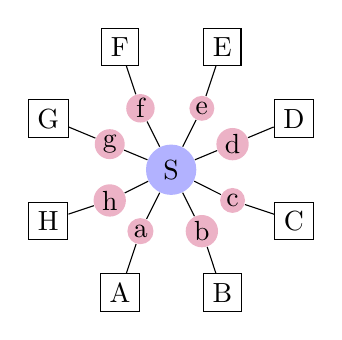
\begin{tikzpicture}[xscale=1.3,yscale=1.3]\normalsize
      \tikzstyle{withshadow}=[draw,drop shadow={opacity=.5},fill=white]
      \tikzstyle{system}=[draw]
      \tikzstyle{standard}=[circle,fill=blue!30]
      \tikzstyle{interface}=[circle,fill=purple!30,inner sep = 1pt,]
      \node[system] (a) at (0,.3) {A};
      \node[system] (b) at (1,.3) {B};
      \node[system] (c) at (1.7,1) {C};
      \node[system] (d) at (1.7,2) {D};
      \node[system] (e) at (1,2.7) {E};
      \node[system] (f) at (0,2.7) {F};
      \node[system] (g) at (-.7,2) {G};
      \node[system] (h) at (-.7,1) {H};
      \node[standard] (m) at (.5,1.5) {S};
      \node[interface] (ia) at (0.2,.9) {a};
      \node[interface] (ib) at (.8,.9) {b};
      \node[interface] (ic) at (1.1,1.2) {c};
      \node[interface] (id) at (1.1,1.75) {d};
      \node[interface] (ie) at (.8,2.1) {e};
      \node[interface] (if) at (0.2,2.1) {f};
      \node[interface] (ig) at (-.1,1.75) {g};
      \node[interface] (ih) at (-.1,1.2) {h};
      \draw (m) -- (ia) -- (a);
      \draw (m) -- (ib) -- (b);
      \draw (m) -- (ic) -- (c);
      \draw (m) -- (id) -- (d);
      \draw (m) -- (ie) -- (e);
      \draw (m) -- (if) -- (f);
      \draw (m) -- (ig) -- (g);
      \draw (m) -- (ih) -- (h);
      \end{tikzpicture}
  \caption{The MiTM Approach to Connecting Systems.}\label{fig:mitmconnect}\vspace*{-1em}
\end{wrapfigure}
The MitM ontology in the center of Figure~\ref{fig:mitmconnect} models the true,
underlying mathematical semantics in \ommt and allows translation between this centrally
formalized knowledge and the systems on the boundary via views and alignments.
This mathematical knowledge is modeled using the well-established theory graph paradigm
and is stored inside our \ommt-based MathHub system~\cite{MathHub:on}. 

The knowledge in the mathematical software systems -- denoted by square boxes in
Figure~\ref{fig:mitmconnect} -- also modeled via \ommt theory graphs the \textbf{API
  theories} -- the corresponding red circles; these are generated from the
knowledge bases in the systems by a custom process. The API theories allow us to implement
translation with the help of \ommt views and alignments between the ontology -- the
Math-In-The-Middle -- and each of the systems and use these translations for transporting
computational tasks between the systems. 

The realization of the MitM approach crucially depends on the information architecture of
the \ommt language~\cite{Kohlhase:OMDoc1.2,RabKoh:WSMSML13} and its implementation in the
\mmt system~\cite{Rabe:MAGMS13,uniformal:on}.

In \ommt knowledge is organized in \textbf{theories}, which contain information about
mathematical concepts and objects in the form of \textbf{declarations}. Theories are
organized into an ``object-oriented'' inheritance structure via \textbf{inclusions} and
\textbf{structures} (for controlled multiple inheritance), which is augmented via
truth-preserving mappings between theories called \textbf{views}, which allow to relate
concepts of pre-existing theories and transport theorems between these. Inclusions,
structures, and views impose a graph structure on the represented mathematical knowledge,
called a \textbf{theory graph}. 

We observe that even very large mathematical knowledge spaces about abstract mathematical
domains can be represented by small, but densely connected, theory graphs, if we make all
inherited material explicit in a process called \textbf{flattening}. The \ommt language
provides systematic names (\mmt URIs) for all objects, properties, and relations in the
induced knowledge space, and given the represented theory graph, the \mmt system can
compute them on demand. 

Generally, knowledge in a knowledge space given by a theory graph loaded by the \mmt system can be accessed by either giving it's \mmt URI, or by uniquely describing it via a set of conditions. 
To achieve the latter, \mmt has a Query Language called QMT~\cite{Rabe:qlfml12}, which allows even complex conditions to be specified. 
Currently, the \mmt system loads the theory graph into main memory at startup and interleaves incremental flattening and query evaluation operations on the \mmt data structures until the result has been produced. 

In \cite{KohMuePfe:kbimss17} we show that the MitM approach, its \ommt-based realization,
and distribution via the SCSCP protocol are sufficient for distributed, federated computation
between multiple computer algebra systems (Sage, GAP, and Singular), and that the MitM
ontology of abstract group theory can be represented in \ommt efficiently. This setup is
effective because
\begin{compactitem}
\item the knowledge spaces behind abstract and computational mathematics can be represented in theory graphs very space-efficiently: The compression factors between a knowledge space and its theory graph -- we call it the \textbf{TG factor} -- exceeds two orders of magnitude even for small domains.
\item only small parts of the knowledge space are traversed for a given computation. 
\end{compactitem}

But the \textsf{OpenDreamKit} VRE must also include mathematical data sources like the \lmfdb or the OEIS, which contain millions of mathematical objects. For such knowledge sources, the classical \mmt system is not yet suitable:
\begin{compactitem}
\item the knowledge space corresponding to the data base content cannot be compressed by ``general mathematical principles'' like inheritance. 
Indeed, redundant information is already largely eliminated by the data base schema and the ``business logic'' of the information system it feeds.
\item typically large parts of the knowledge space need to be traversed to obtain the intended results to queries.
\end{compactitem}
Therefore, we extend the concept of \ommt theories -- which carry the implicit assumption of containing only a small number of declarations (see~\cite{FaGu:lt92} for a discussion) -- to \textbf{virtual theories}, which can have an unlimited (possibly infinite) number of declarations. 
To contrast the intended uses we will call the classical \ommt theories \textbf{concrete theories}.  
In practice, a virtual theory is represented by concrete approximations: \ommt works with
a concrete theory, whose size changes dynamically as a suitable backend infrastructure
generates declarations on demand.
\end{oldpart}

\subsection{Mathematical Knowledge Bases}\label{sec:mkb}
\begin{oldpart}{MK: copied here from the MACIS-interop paper, needs to be adapted.}
  There are various large-scale sources of mathematical knowledge.  These include
\begin{compactitem}
\item generic information systems like Wikipedia,
\item collections of informal but rigorous mathematical documents -- e.g. research libraries, publisher's ``digital libraries'', or the Cornell preprint arXiv,
\item literature information systems like zbMATH or MathSciNet,
\item databases of mathematical objects -- like the GAP group libraries, the Online Encyclopedia of Integer sequences (OEIS~\cite{Sloane:OEIS,oeis}), and the L-Functions and Modular Forms Database (LMFDB~\cite{Cremona:LMFDB16,lmfdb:on}),
\item fully formal theorem prover libraries like those of Mizar, Coq, PVS, and the HOL systems.
\end{compactitem}
  
We will use the term \textbf{mathematical knowledge bases} to refer to them collectively and restrict ourselves to those that are available digitally.
They are very useful in mathematical research, applications, and education.  
Commonly these systems are only accessible via a dedicated web interface that allows humans to query or browse the databases. 
A programmatic interface, if it exists at all, is usually system specific, to use it, users need to be familiar both with the mathematical background and internal structure of the system in question.  
No predominant standard exists, and these interfaces usually only expose the low-level raw database content.
We claim that mathematicians and other scientists desire a ``programmatic, mathematical API'' that gives access to the knowledge-bases programmatically via their mathematical constructions and properties. 
We focus on addressing this problem in this paper. 

For our implementation we interpret mathematical knowledge bases as \ommt theory graphs -- modular, flexi-formal representations of mathematical objects, their properties, and relations. 
This embedding gives us a common conceptual framework to handle different knowledge sources, and the modular and heterogeneous nature of \ommt theory graph can be used to reconcile differing ontological commitments of the knowledge sources with in this conceptual framework.

To cope with the scale of common mathematical knowledge bases we generalize \ommt theories to ``virtual theories'', which allow for unlimited, dynamically growing number of declarations.
We also update the knowledge management algorithms in the \mmt system so that they can directly deal with the databases underlying the knowledge bases.
Here we provide a systematic solution for encoding/decoding between low-level representations in standard databases and high-level mathematical representations.

This paper proceeds as follows: 
In Section~\ref{sec:mmtmitm} we give a short overview of \ommt theory graphs along with the Math-In-The-Middle approach developed in the \textsf{OpenDreamKit} project, our primary use-case for virtual theories. 
Section~\ref{sec:sota} discusses \lmfdb and its interface as an example of a very large state-of-the-art mathematical knowledge base, and Section~\ref{sec:vt} shows how it can be represented as a set of virtual theories. 
Section~\ref{sec:access} introduces the codec architecture and describes how to access virtual theories at the semantic/mathematical level, and Section~\ref{sec:qmt} makes QMT queries aware of virtual theories. 
Section~\ref{sec:concl} concludes the paper.
\end{oldpart}

%%% Local Variables:
%%% mode: latex
%%% TeX-master: "report"
%%% End:

% LocalWords: sec:mitm Jupyter jupyter-project:on KohDavGin:psewads11 BusCapCar:2oms04
% standardization DehKohKon:iop16 textbf RabKoh:WSMSML13,uniformal:on MueGauKal:cacfms17
% sec:apit serialize normalizer mathcal compute-the-normalizer MitM-based centering
% mitmcomm MueRoYuRa:abtafs17 Rabe:MAGMS13,uniformal:on inparaenum Sagey lstlisting scscp
% mmt,is_cyclic scscp lmfdb mmt,query transitivegroup lstinline gap,is_cyclic,scscp
% lmfdb,query synthesizes mathescape Sageify mathtt ldots,X_n Gonthier LocalWords:
% wrapfigure vspace tikzinput mistargraph fig:mitm mitm_poc emph mcpoot13 LocalWords:
% formalizations optimizations standardized serializer oldpart behavior LocalWords:
% itemized
